\section{Verification episodes}\label{app:verification}

This section documents the three cases mentioned in Section~\ref{sec:protocol} and reports the measured hiddenness.

\textbf{Numerical ``transient chaos'' in the Chua circuit.} With RK4 at $\Delta t=0.01$, all 256 copies of a state on the hidden chaotic set of Chua~I converge within $t\le2\times10^4$ to a spurious periodic orbit of the same size (median time about 1500; Figure~\ref{fig:chuatrans}a). At $\Delta t=0.0025$, none of 96 copies leaves the set before $t=10^4$, and DOP853 preserves the chaos up to $t=4000$. At $\Delta t=0.01$, the fractions of the hidden attractors are underestimated almost twofold (Figure~\ref{fig:chuatrans}b). For a piecewise-linear system, this is an integrator artifact and the mirror image of the spurious ``hidden Lorenz attractor''~\cite{Munmuangsaen2018,SprottMunmuangsaen2018Comment}: there, transient chaos was mistaken for an attractor; here, an attractor is mistaken for transient chaos. The step-convergence check is therefore mandatory.

\textbf{Basin fractions of the Chua circuit.} Two independent implementations, Python (RK4, $\Delta t=0.0025$) and Attractors.jl (Vern9), give fractions that agree to within 0.01 in the balls of radius $r=3$ and $r=5$ and in Zelinka's box. Neither of them reproduces Table~1 of the review in Ref.~\cite{GuanXie2025} (Table~\ref{tab:chuafrac}). In the ball $r=3$, the escape fraction is 0.19 in our computations versus 0.06 in the review, the fraction of F$_0$ is 0.44 versus 0.75, and that of each hidden attractor is 0.18 versus 0.095. The last pair is suggestive: our fractions of the hidden attractors at the coarse step $\Delta t=0.01$ are also about 0.09 (Figure~\ref{fig:chuatrans}b), so the review's hidden-attractor fractions are consistent with the artifact above, whereas its escape and F$_0$ fractions remain unexplained. The basin structure in the plane $z=0$ coincides with that of the review and of the catalog of Ref.~\cite{Wagemakers2025Zoo} (Figure~\ref{fig:chuaI}).

\textbf{Intermittency and transient sets.} In NE4, the ``second attractor'' found by a preliminary version of the protocol turned out to be intermittency of the single chaotic attractor; this was fixed by the observation window $T_{\rm obs}=500\gg1/\lambda$. The transient chaos of the Lorenz system $(4,29,2)$ lives for about $10^4$ time units: all eight copies decay at times $t\le7\times10^4$. A protocol with an observation window shorter than the lifetime would accept this set as an attractor (Figure~\ref{fig:verif}). The Rabinovich set at $r=6.8$ lives longer than $10^5$ time units for six of eight copies, consistent with the estimate $\tau\sim5\times10^7$ of Ref.~\cite{SprottMunmuangsaen2018Comment}; in the benchmark, it is used only as a control.

\textbf{Hiddenness measure.} Table~\ref{tab:hidden} lists $h_\varepsilon$ for the systems with equilibria. For SE3 and SE11, $h_\varepsilon=0$ at all three scales. For Chua~I, $h_\varepsilon$ grows from 0 at $\varepsilon=10^{-3}L$ through 0.003 ($10^{-2}L$) to 0.19 ($10^{-1}L$). For the Rabinovich system at $r=100$, the values are 0, 0.03, and 0.65: the attractor is hidden only in the strict limit $\varepsilon\to0$, and already at $\varepsilon=10^{-2}L$, trajectories from the neighborhood of an equilibrium enter its basin. The binary definition thus does not distinguish between ``deeply'' and ``shallowly'' hidden attractors, whereas $h_\varepsilon$ does. For the Jafari chaos, copies with a perturbation of $10^{-3}$ escape (Figure~\ref{fig:verif}), whereas all 32 copies with a perturbation of $10^{-6}$ stay on the attractor for $10^4$ time units with RK4, and so do eight copies with DOP853; their finite-time exponents are $0.056\pm0.011$, none below 0.01. It is therefore an attractor whose basin is thinner than a relative distance of $10^{-3}$ near the attractor, not a long transient.

A measured zero of $h_\varepsilon$ is informative only relative to the number of starts $n$: with no hits, $h_\varepsilon<3/n$ at the 95\% level, so each zero in Table~\ref{tab:hidden} only bounds $h_\varepsilon$ by $3/n$ for the $n$ given there. For rare targets with $p$ comparable to $3/n$, a zero does not by itself separate ``hidden'' from ``rare.'' For SE11, Chua~II, and the rare family of the coupled Chua circuits, $h_\varepsilon$ was therefore remeasured with $2\times10^5$ starts per radius: no start reaches a hidden target at $10^{-3}L$ or $10^{-2}L$, so $h_\varepsilon<1.5\times10^{-5}$ at the 95\% level, below the basin measures of all three targets (Section~\ref{sec:coupled}).

\textbf{The line of equilibria of LE1.} The measure $h_\varepsilon$ is defined for isolated equilibria; for LE1 we started trajectories near the points $(0,0,z_0)$ of the line, for 140 values of $z_0\in[-3,4]$ ($z_0=0$ excluded), in 24 random directions at distances $10^{-8}$ and $10^{-4}$, and integrated them by RK4 ($\Delta t=0.005$) for 600 time units. A start counts as a hit if it stays within 0.05 of a reference orbit on the attractor in at least 90 of the last 100 checks. No start near the stable part of the line ($z_0<0$) reaches the attractor. Near the unstable part, 170 of the 3360 starts at distance $10^{-8}$ (175 at $10^{-4}$) reach it, all from $0.35\le z_0\le2.2$, where up to all starts of a single $z_0$ reach it; the other starts return to the line (1762) or escape (1404). The attractor is therefore excited from the unstable equilibria of the line and hidden only with respect to its stable part, as noted by Jafari and Sprott~\cite{JafariSprott2013}.

% Proposed caption (replaces the bar chart fig04_table1_comparison / \ref{fig:table1}):
% Basin fractions of Chua~I under uniform sampling in balls of radius $r=3$ and $r=5$ about the origin: escape to infinity ($\infty$), the stable equilibrium F$_0$, and the two symmetric hidden attractors A and B. Sources: Table~1 of the review in Ref.~\cite{GuanXie2025} and two independent implementations, Python (RK4, $\Delta t=0.0025$, $10^5$ points per ball) and Attractors.jl (Vern9, $10^4$ points per ball). The two implementations agree with each other but not with the review. In the implementations, A and B are matched by the sign of the mean of $x$ on the attractor; for the review, they are listed in the order of its Table~1. The fraction of unmatched trajectories in the Python run (0.06\%) is omitted.

\begin{table}[tbhp]
\centering
\caption{Basin fractions of Chua~I under uniform sampling in balls of radius $r=3$ and $r=5$ about the origin: escape to infinity ($\infty$), the stable equilibrium F$_0$, and the two symmetric hidden attractors A and B. Sources: Table~1 of the review in Ref.~\cite{GuanXie2025} and two independent implementations, Python (RK4, $\Delta t=0.0025$, $10^5$ points per ball) and Attractors.jl (Vern9, $10^4$ points per ball). The two implementations agree with each other but not with the review. In the implementations, A and B are matched by the sign of the mean of $x$ on the attractor; for the review, they are listed in the order of its Table~1. The fraction of unmatched trajectories in the Python run (0.06\%) is omitted.}
\label{tab:chuafrac}
\scriptsize
\setlength{\tabcolsep}{3pt}

\begin{tabular}{lrrrrrrrr}
\toprule
 & \multicolumn{4}{c}{$r=3$} & \multicolumn{4}{c}{$r=5$} \\
Source & $\infty$ & F$_0$ & A & B & $\infty$ & F$_0$ & A & B \\
\midrule
Ref.~\cite{GuanXie2025}, Table~1 & 0.06 & 0.75 & 0.09 & 0.10 & 0.23 & 0.50 & 0.14 & 0.13 \\
Python, RK4 & 0.19 & 0.44 & 0.18 & 0.18 & 0.55 & 0.18 & 0.14 & 0.14 \\
Attractors.jl & 0.19 & 0.44 & 0.18 & 0.19 & 0.55 & 0.18 & 0.13 & 0.14 \\
\bottomrule
\end{tabular}

\end{table}


% Proposed caption (replaces the plot fig40_hiddenness / \ref{fig:hidden}):
% Hiddenness measure $h_\varepsilon$: the fraction of trajectories started in the $\varepsilon$-neighborhoods of the equilibria (uniformly in the ball of radius $\varepsilon$ about each equilibrium, plus the two points $e\pm\varepsilon u$ along every unstable eigendirection $u$) that enter the basin of the attractor, for $\varepsilon=10^{-3}L$, $10^{-2}L$, and $10^{-1}L$, where $L$ is the half-width of the region $B$; $n$ is the number of starts per radius. An entry of 0 means no hit among the $n$ starts (95\% upper bound $3/n$). For Chua~I, the two hidden attractors are listed separately, and the values quoted in the text are the sums over A and B; for Chua~II, the row ``chaos'' refers to one of the two symmetric chaotic attractors. The Lorenz transient set is shown for comparison.
% Data caveat (results/e11_hiddenness.json): the reference set of this experiment contains one chaotic attractor of Chua II
% (new1) and the cycle LC (new0); at eps = 1e-1 L, 103 of 1202 starts (8.6%) reach an unmatched regime, presumably the
% symmetric second chaotic attractor, so h for "chaos, both" would be about 0.18. Wang--Chen #2 at 1e-1 L: 2 unmatched, 1% escape.
% Hits behind the nonzero entries: Chua I A 3/101, B 1/122 (1e-2 L / 1e-1 L); Chua II LC 484, chaos 115; Rabinovich 39/781;
% Lorenz 49.

\begin{table}[tbhp]
\centering
\caption{Hiddenness measure $h_\varepsilon$: the fraction of trajectories started in the $\varepsilon$-neighborhoods of the equilibria (uniformly in the ball of radius $\varepsilon$ about each equilibrium, plus the two points $e\pm\varepsilon u$ along every unstable eigendirection $u$) that enter the basin of the attractor, for $\varepsilon=10^{-3}L$, $10^{-2}L$, and $10^{-1}L$, where $L$ is the half-width of the region $B$; $n$ is the number of starts per radius. An entry of 0 means no hit among the $n$ starts (95\% upper bound $3/n$). For Chua~I, the two hidden attractors are listed separately, and the values quoted in the text are the sums over A and B; for Chua~II, the row ``chaos'' refers to one of the two symmetric chaotic attractors. The Lorenz transient set is shown for comparison.}
\label{tab:hidden}
\scriptsize

\begin{tabular}{lrrrr}
\toprule
System, attractor & $n$ & $\varepsilon=10^{-3}L$ & $10^{-2}L$ & $10^{-1}L$ \\
\midrule
Chua I, A & 1204 & 0 & 0.00249 & 0.0839 \\
Chua I, B & 1204 & 0 & 0.000831 & 0.101 \\
Chua II, cycle LC & 1202 & 0 & 0 & 0.403 \\
Chua II, chaos & 1202 & 0 & 0 & 0.0957 \\
Wang--Chen \#2 & 400 & 0 & 0 & 0.838 \\
SE3 & 400 & 0 & 0 & 0 \\
SE11 & 400 & 0 & 0 & 0 \\
Rabinovich, $r=100$ & 1202 & 0 & 0.0324 & 0.650 \\
Lorenz $(4,29,2)$, transient set & 1202 & 0 & 0 & 0.0408 \\
\bottomrule
\end{tabular}

\end{table}


\begin{figure}[tbhp]
\centering
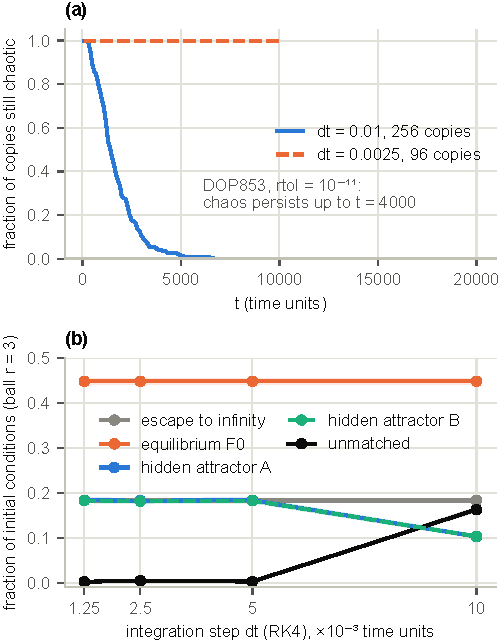
\includegraphics[width=0.62\textwidth]{figures/fig02_chua_transient.pdf}
\caption{Numerical ``transient chaos'' in Chua~I. (a) The fraction of copies (initial perturbation $10^{-3}$) remaining on the hidden chaotic set. With RK4 at $\Delta t=0.01$, the chaos decays onto a spurious periodic orbit; at $\Delta t=0.0025$, it persists to the end of the window. (b) Basin fractions versus the RK4 step (ball $r=3$, $2\times10^4$ points, $T_{\rm tr}=1000$). At $\Delta t=0.01$, about 16\% of trajectories land on the spurious orbit (``unmatched''), and the fractions of the hidden attractors are underestimated. For $\Delta t\le0.005$, the fractions stabilize.}
\label{fig:chuatrans}
\end{figure}

\begin{figure}[tbhp]
\centering
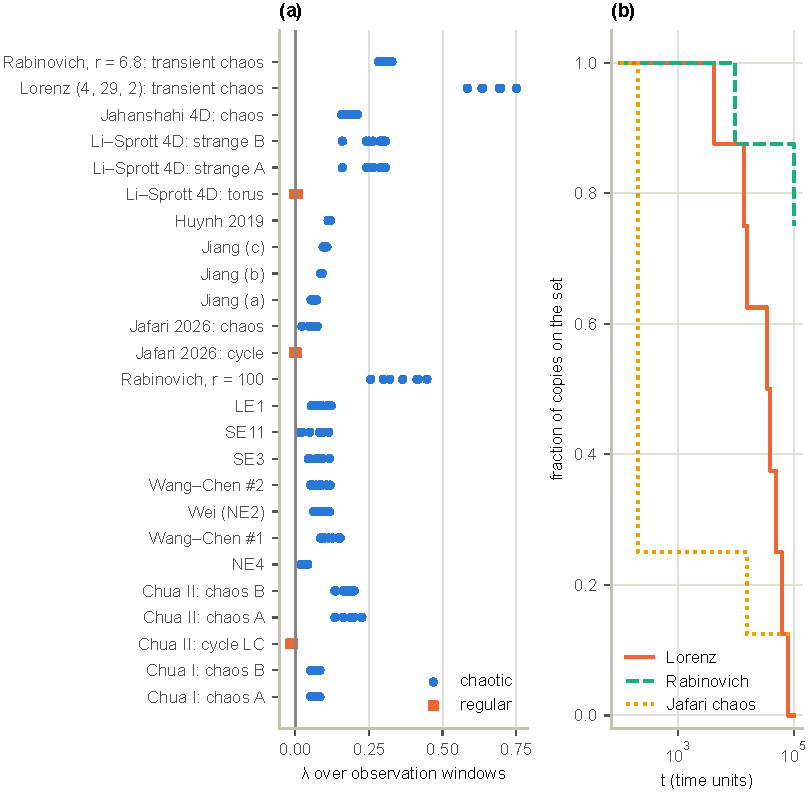
\includegraphics[width=\textwidth]{figures/fig41_verification.pdf}
\caption{Verification of the targets. (a) The largest Lyapunov exponent over consecutive observation windows for all targets of the benchmark; blue: chaotic regimes; orange: regular ones (the cycle LC of Chua~II, the Jafari cycle, and the Li--Sprott torus). (b) Lifetime check over long times (eight copies with initial perturbation $10^{-3}$). The Lorenz transient chaos decays completely. For the Rabinovich set at $r=6.8$, six of eight copies survive to $10^5$. For the fragile Jafari chaos, six of eight copies escape to infinity already by $t=200$: with a relative perturbation of $10^{-3}$, the copies leave its thin basin; with $10^{-6}$, all of them stay on the attractor (Section~\ref{app:verification}).}
\label{fig:verif}
\end{figure}

